\documentclass{article}
\usepackage{tikz}

\usetikzlibrary{matrix,arrows,fit}
\tikzset{circarrow/.style={
		*->,
		shorten <=-2pt
	}
}

\begin{document}
\leavevmode\vadjust{\vspace{-\baselineskip}}\newline
\begin{center}
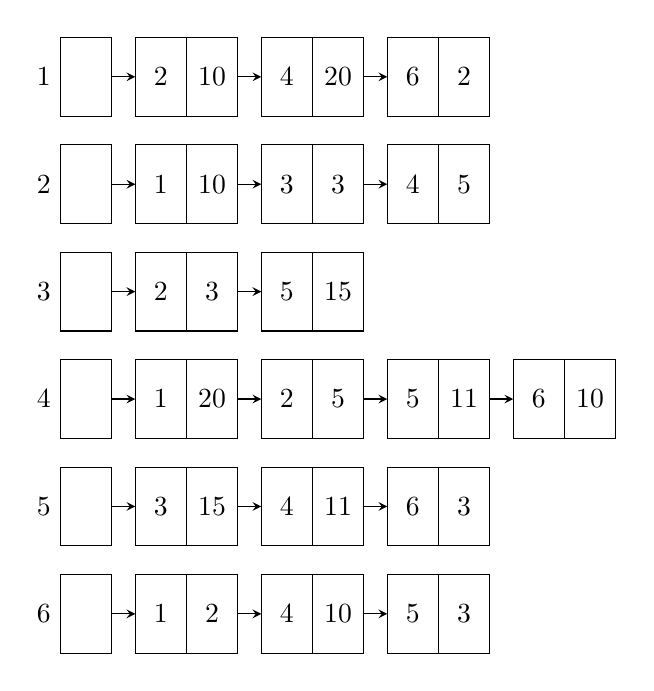
\begin{tikzpicture}[>=stealth]
\matrix (M)
[
	matrix of nodes,
	column sep=-\pgflinewidth,
	row sep=3.5mm,
	nodes in empty cells,
	nodes= {
		draw, minimum width=.65cm, outer sep=0pt,
		minimum height=1.0cm, anchor=center
	}
] {
 &[3mm] 2 & 10 &[3mm] 4 & 20 &[3mm] 6 & 2 \\
 & 1 & 10 & 3 & 3 & 4 & 5 \\
 & 2 & 3 & 5 & 15 \\
 & 1 & 20 & 2 & 5 & 5 & 11 &[3mm] 6 & 10 \\
 & 3 & 15 & 4 & 11 & 6 & 3 \\
 & 1 & 2 & 4 & 10 & 5 & 3 \\
};

\foreach \i in {1,2,3,4,5,6} {
	\path (M-\i-1) [late options={label=left:\i}];
	\draw[->] (M-\i-1)--(M-\i-2.west);
	\draw[->] (M-\i-3)--(M-\i-4.west);
}
\draw[->] (M-1-5)--(M-1-6.west);
\draw[->] (M-2-5)--(M-2-6.west);
\draw[->] (M-4-5)--(M-4-6.west);
\draw[->] (M-4-7)--(M-4-8.west);
\draw[->] (M-5-5)--(M-5-6.west);
\draw[->] (M-6-5)--(M-6-6.west);
\end{tikzpicture} 
\end{center}
\end{document}

